\chapter{Results}


\section{Arduino: Euler angle output}
Based on the information presented in List~\ref{lst:time-consuming} (see Appendix) in the case of using four IMUs, the data collection interval of each round was about 55ms, nearly 20hz.

Meanwhile, it also turned out that the output of yaw axis data was unstable and inaccurate.
Due to the time limitation, such data was discarded, leading to a loss of some functions for this project.
As a replacement, the roll axis data was used to identify the pitch angle, which has been illustrated in the data mapping part of~\ref{subsec:engine}.

\section{Displaying engine: flexible configuration}\label{sec:flexible}
\begin{figure}[htbp]
	\centering
	\begin{subfigure}[b]{0.45\textwidth}
		\centering
		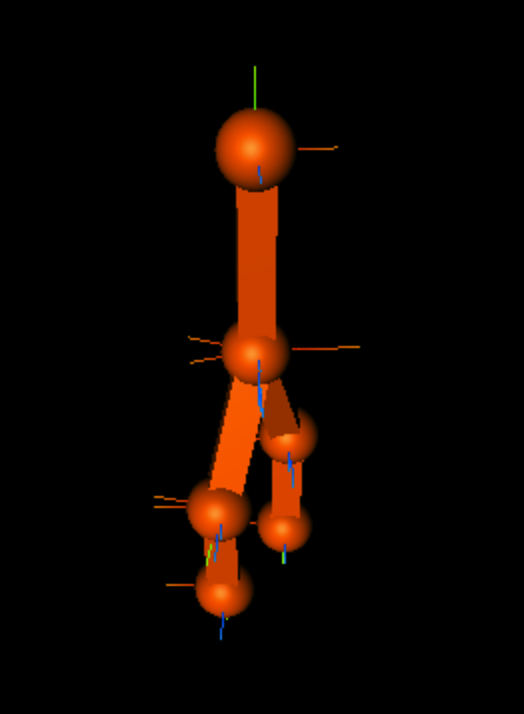
\includegraphics[width=0.8\textwidth]{
			fileForWriting/ouput-model}
		\caption[The model generated by the input text for human lower body]{A human lower body model generated by the input text in List~\ref{lst:lower-body-config}.}
		\label{fig:lower-body-model}
	\end{subfigure}
	\hfill
	\begin{subfigure}[b]{0.45\textwidth}
		\centering
		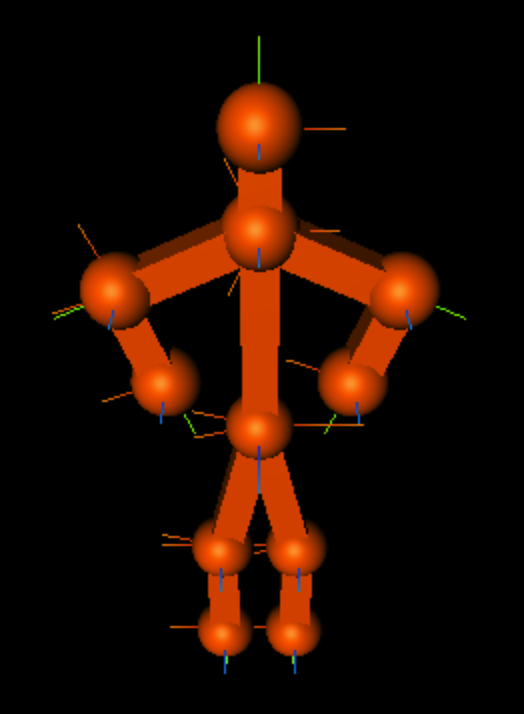
\includegraphics[width=0.8\textwidth]{
			fileForWriting/full-body}
		\caption[The model generated by the input text for a full human body]{A full human body model generated by the input text in List~\ref{lst:full-body-config}.}
		\label{fig:full-body-model}
	\end{subfigure}
	\caption[]{Corresponding models generated by various text inputs in the displaying engine.}
	\label{fig:flexible-input}
\end{figure}

As depicted in Figure~\ref{fig:flexible-input}, with different text inputs, the displaying engine could generate corresponding models.
The Figure (b) is based on the input of Figure (a) but adds other parts such as arms, forearms.
Relevant configs are in List~\ref{lst:lower-body-config} and  List~\ref{lst:full-body-config}.




\section{Displaying engine: asynchronously fetching data}\label{sec:async}
As highlighted by the representation of Figure~\ref{fig:0.73-size}, the thread for data fetching needed about 2 frame intervals to obtain the whole 0.73 MB data from the server.

%-----------This is a FIGURE-----------------------
\begin{figure}[htbp]
	\centering
	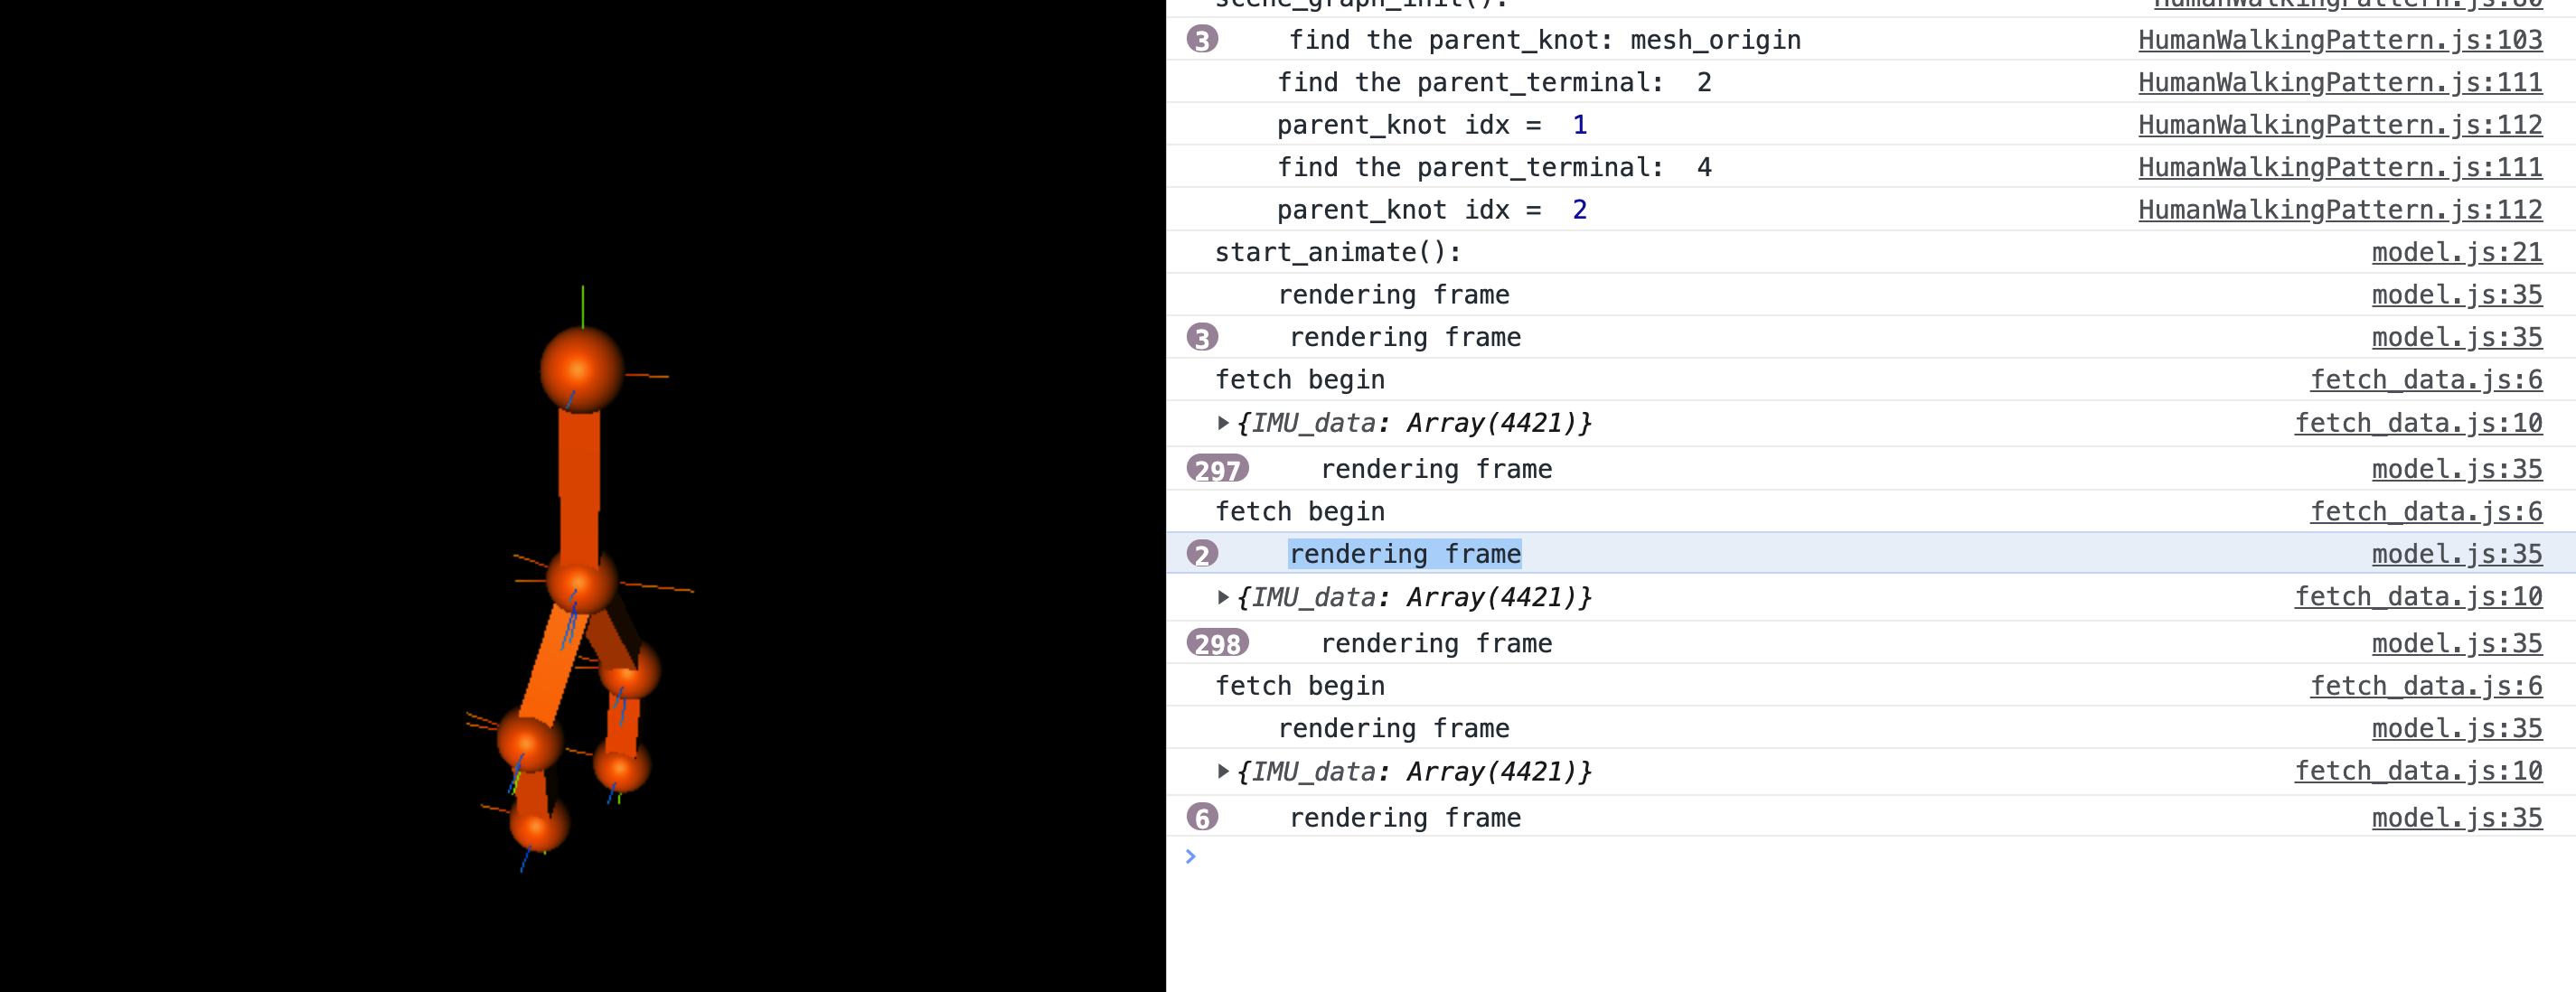
\includegraphics[width=0.9\textwidth]{
		fileForWriting/1mb-test}
	\caption[Time consuming while receiving a single message with a size of 0.73 MB]{Time consuming while fetching a single string message with a size of 0.73 MB. The quantity of poses in such message is 4421.}
	\label{fig:0.73-size}
\end{figure}
%--------End of this FIGURE -----------

By comparison, the thread needed 42 frame intervals to completely hold a 14.4 MB message.

%-----------This is a FIGURE-----------------------
\begin{figure}[htbp]
	\centering
	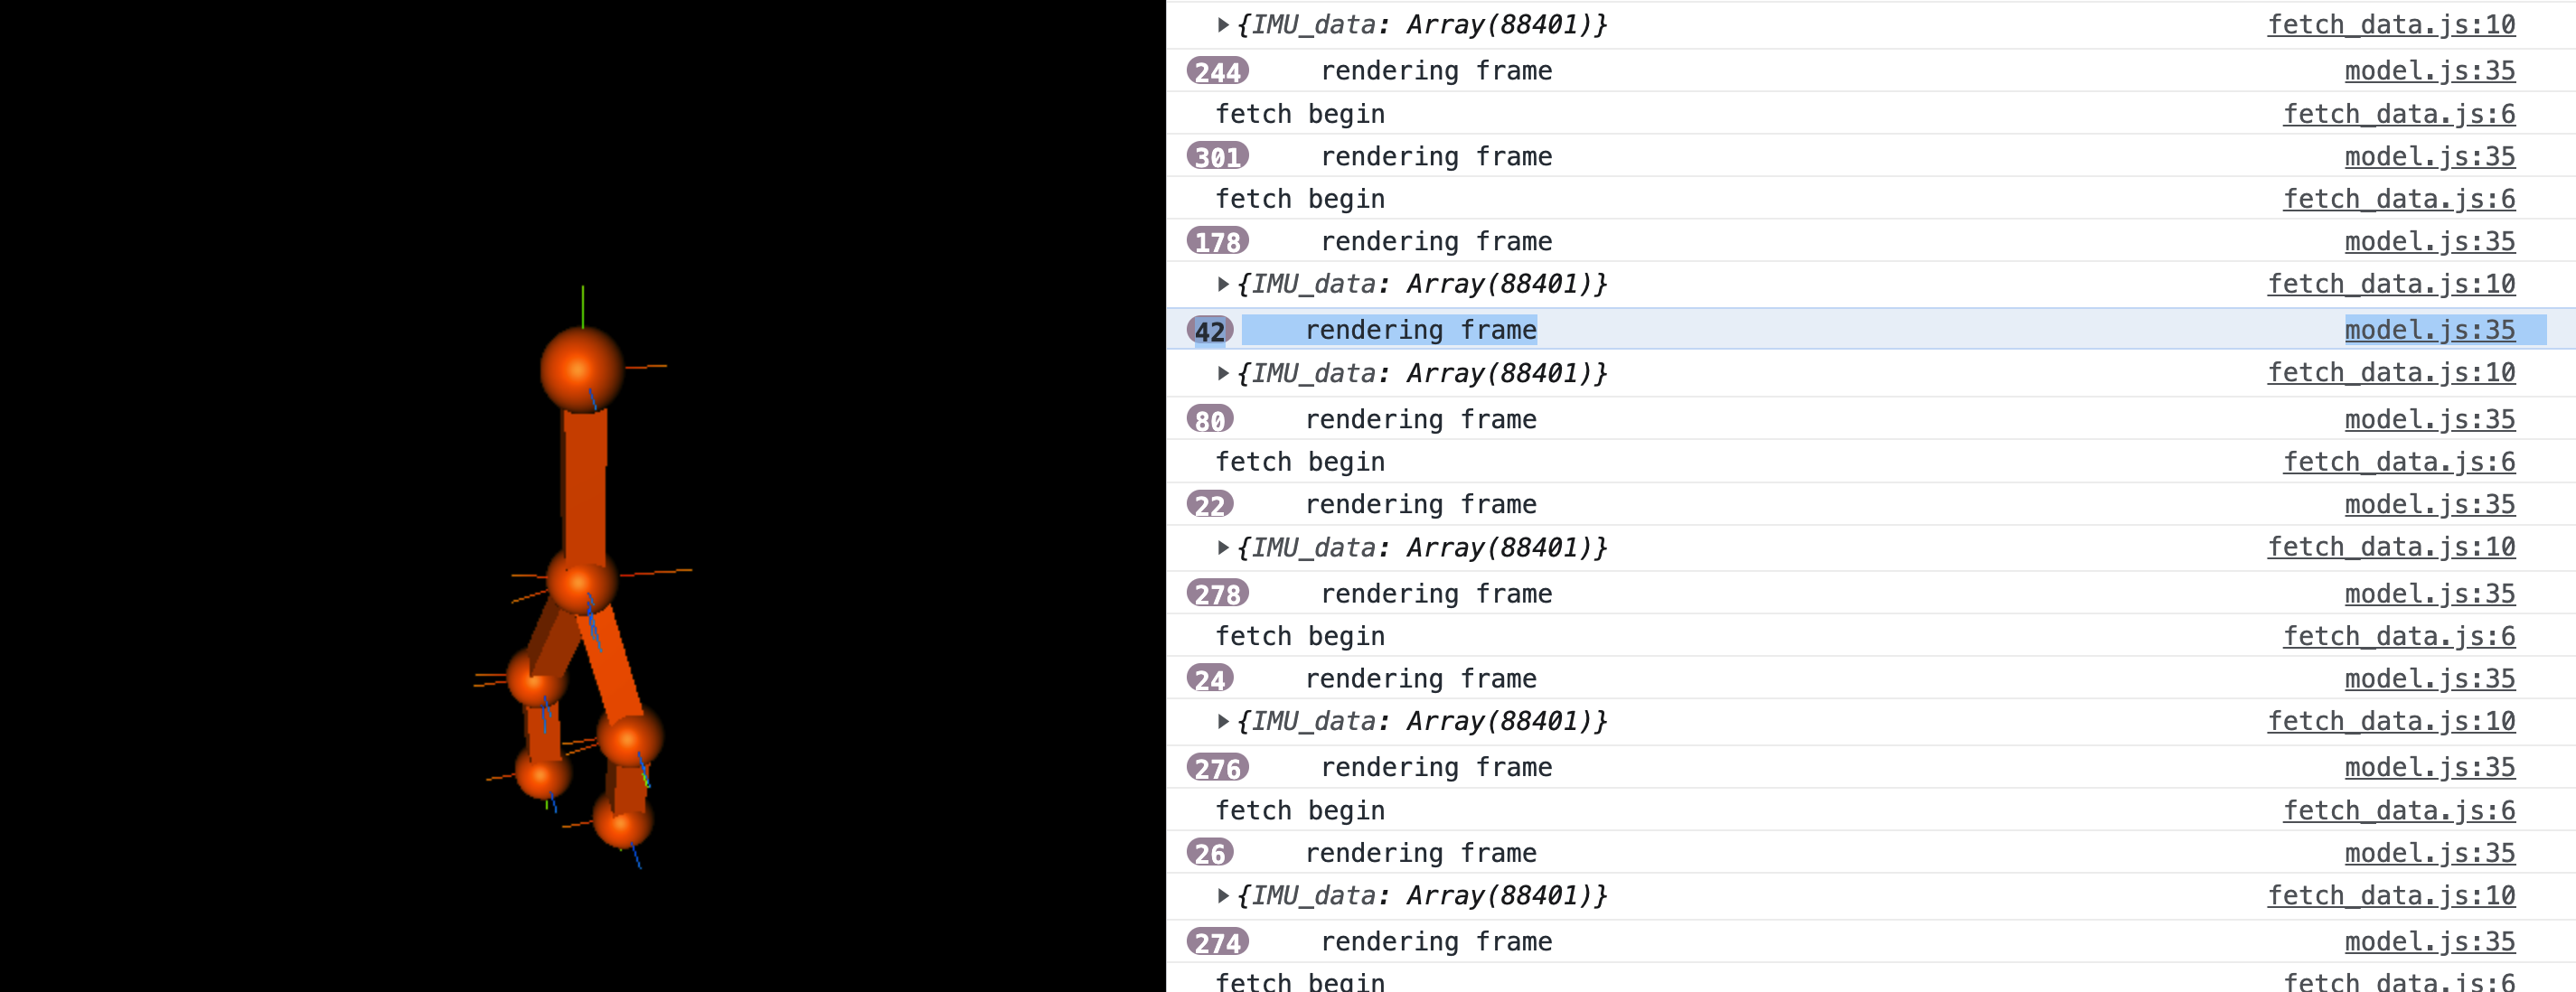
\includegraphics[width=0.9\textwidth]{
		fileForWriting/14mb-test}
	\caption[Time consuming while receiving a single message with a size of 14.4 MB]{Time consuming while fetching a single string message with a size of 14.4 MB. The quantity of poses in such message is 88401.}
	\label{fig:14-size}
\end{figure}
%--------End of this FIGURE -----------

\section{Final Performance}

%-----------This is a FIGURE-----------------------
\begin{figure}[htbp]
	\centering
	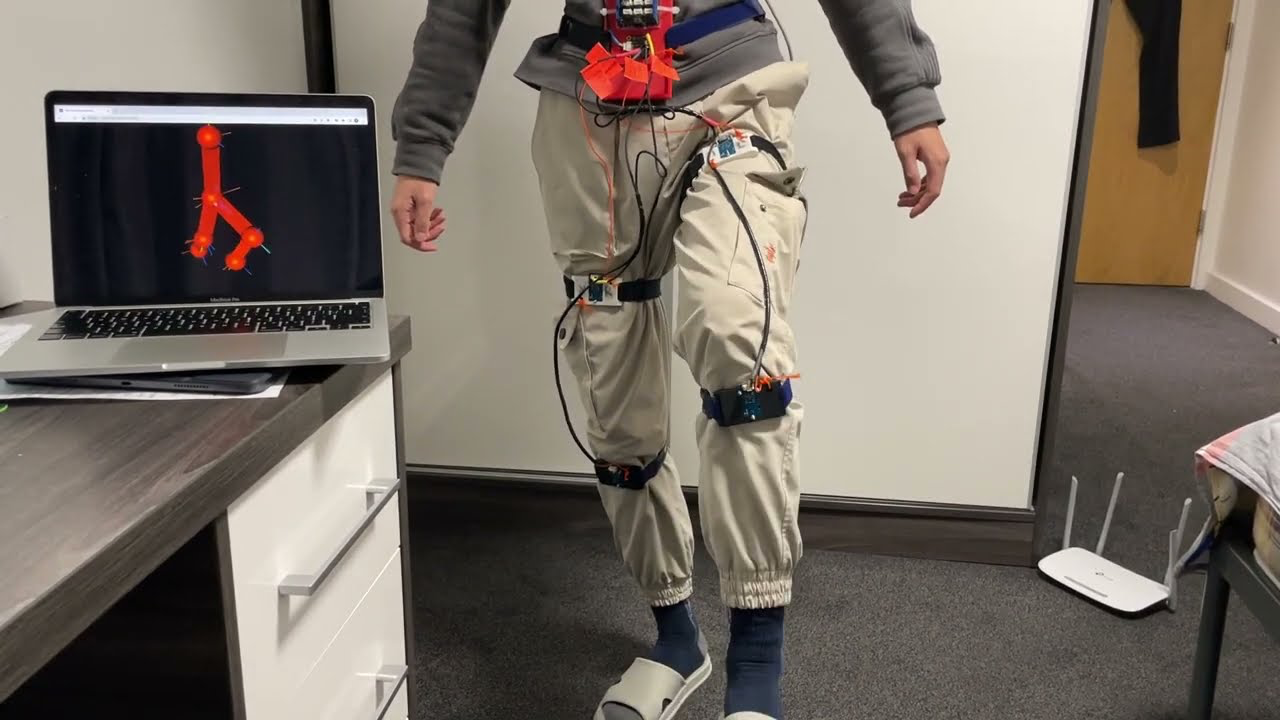
\includegraphics[width=1\textwidth]{
		fileForWriting/youtube-page}
	\caption[A full testing with four IMUs and wireless communication]{A full testing with four IMUs and wireless communication.}
	\label{fig:youtube-demo}
\end{figure}
%--------End of this FIGURE -----------


As presented in the videos at~\cite{youtube-demo},
available via the QR codes in the
footnote\footnote{
\includegraphics[width=1.4cm]{fileForWriting/qrcode-youtube}\cite{youtube-demo}.},
the model generated by the displaying engine in the browser was capable of mimicking human leg movements such as lifting the leg forward or stretching it backward.
As a result, the rotation of the leg could also be recognized and displayed, although it was not well demonstrated in the video.
However, movements of extending the leg to the left or right could not be replicated to the digital twin due to the lack of yaw axis data.

After one-fold interpolation, the animation's rendering rate could reach up to 40 frames per second (FPS)\@.
However, due to potential factors such as communication delays in wireless transmission, the latency between the digital twin and the actual object is still within the range of human perception, approximately 100 ms by estimation.

In addition to the aforementioned results, the inclusion of the threshold operation has also partially reduced the jittering phenomenon in the animation.
However, it was also found that as soon as the distance between the Arduino and the router exceeds two or three meters, there would be a significant increase in delay, which eventually leads to the displaying engine getting stuck.


